\subsection{\textcolor{gray}{Detail of Design}}
The Smart Lock prototype consists of both hardware and software components, designed to provide secure, remote access control with user authentication and cloud connectivity.

\subsubsection{\textcolor{teal}{System Overview}}

Our system integrates a physical keypad-based lock with Wi-Fi-enabled remote access through a mobile application. Users can authenticate using a PIN or biometric authentication (fingerprint or facial recognition), and manage access remotely.

\begin{figure}[h]
    \centering
    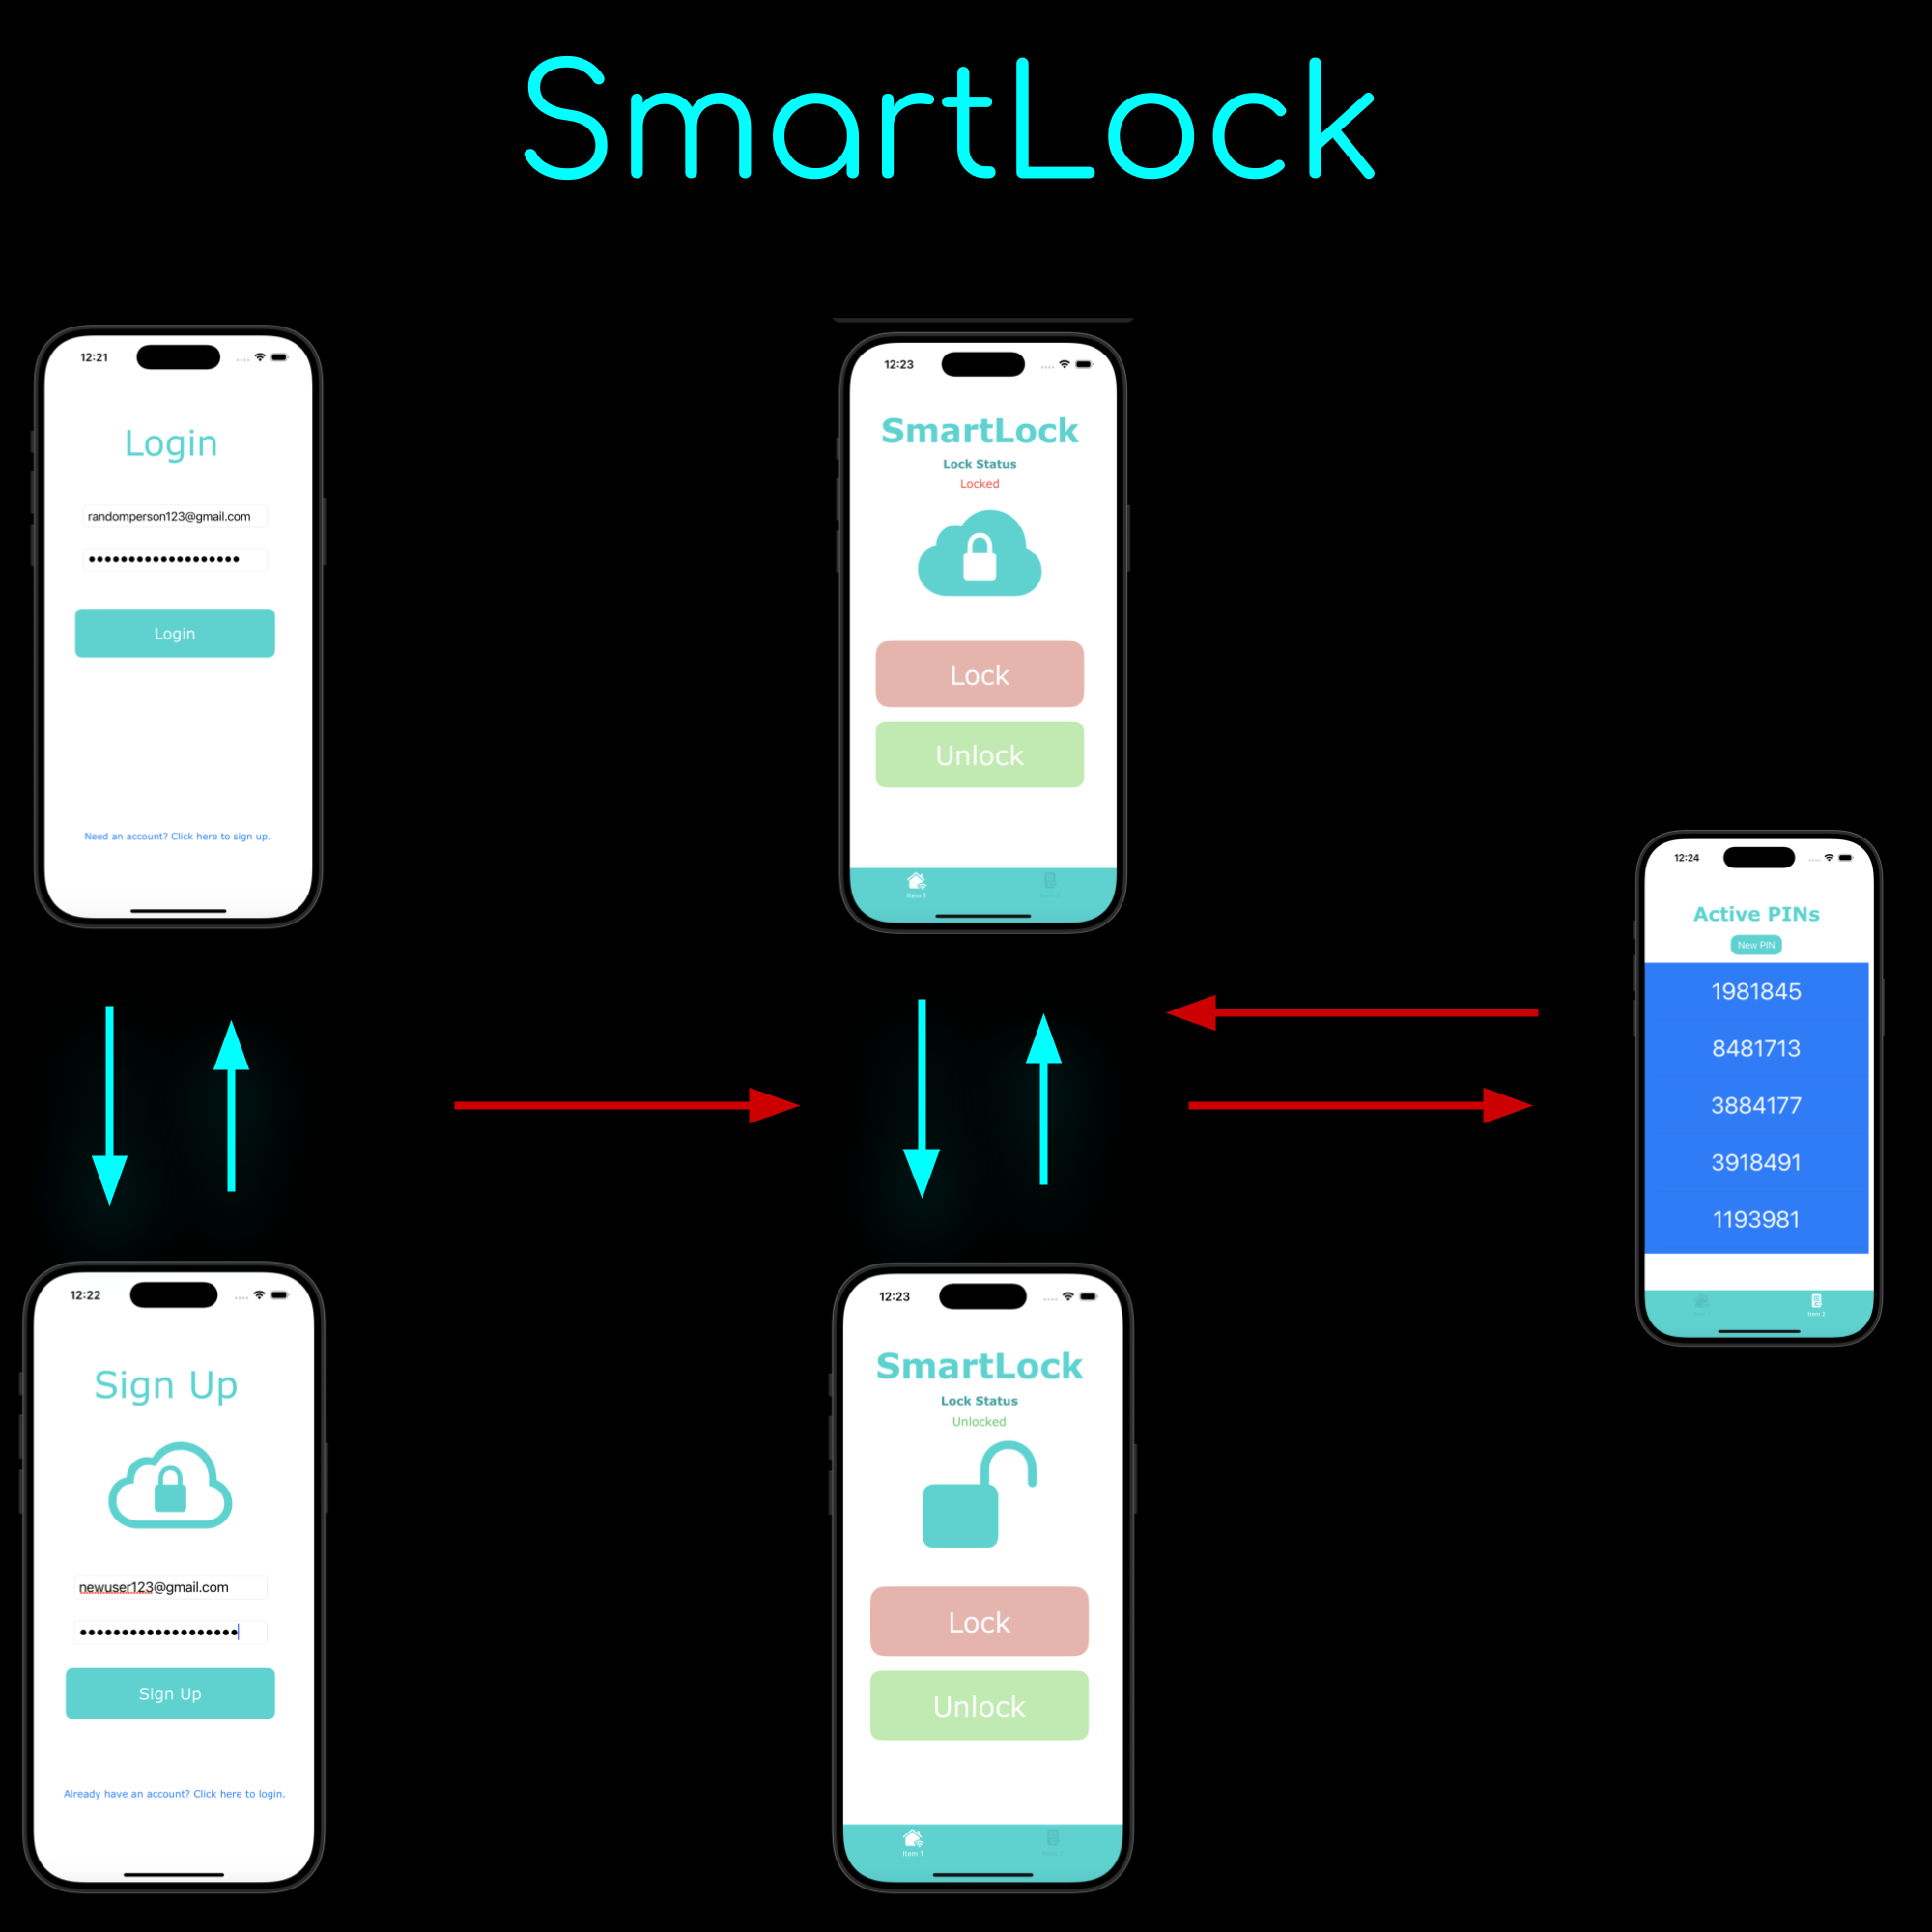
\includegraphics[width=0.65\textwidth]{flowsl.png}
    \caption{Mobile App Flowchart for Smart Lock System}
\end{figure}

\begin{itemize}
    \item Users log in or create an account to access the smart lock.
    \item The main control screen provides lock/unlock buttons.
    \item Users can view and manage active PIN codes for secure access.
    \item The system communicates with a cloud database (Firestore) for real-time authentication and remote control.
\end{itemize}

\subsubsection{\textcolor{teal}{Connectivity and Cloud Integration}}